%----------------------------------------------------------------------------------------
% PACKAGES AND DOCUMENT CONFIGURATIONS
%----------------------------------------------------------------------------------------

  \documentclass[12pt]{article}

  \usepackage{hyperref}
  \usepackage{fancyhdr} % Required for custom headers
  \usepackage{lastpage} % Required to determine the last page for the footer
  \usepackage{extramarks} % Required for headers and footers
  \usepackage[usenames,dvipsnames]{color} % Required for custom colors
  \usepackage{graphicx} % Required to insert images
  \usepackage{listings} % Required for insertion of code
  \usepackage{courier} % Required for the courier font
  \usepackage{lipsum} % Used for inserting dummy 'Lorem ipsum' text into the template
  \usepackage{wrapfig}
  \usepackage{color}
  \usepackage{lscape}

  \setlength\parindent{0pt} % Removes all indentation from paragraphs
  \renewcommand{\labelenumi}{\alph{enumi}.} % Make numbering in the itemize environment by letter rather than number (e.g. section 6)

  % Margins
  \topmargin=-0.4in
  \evensidemargin=0.2in
  \oddsidemargin=-0.2in
  \textwidth=7.0in
  \textheight=9.0in
  % \headsep=0.25in

  % \linespread{1.1} % Line spacing

  \definecolor{dkgreen}{rgb}{0,0.6,0}
  \definecolor{gray}{rgb}{0.5,0.5,0.5}
  \definecolor{mauve}{rgb}{0.58,0,0.82}
  \definecolor{greyish}{rgb}{0.96,0.96,0.96}

  \lstset{
    backgroundcolor=\color{greyish},   % choose the background color; you must add \usepackage{color} or \usepackage{xcolor}
    frame=tblr,
    numbers=left,                       % where to put the line-numbers; possible values are (none, left, right)
    numbersep=5pt,                   % how far the line-numbers are from the code
    numberstyle=\tiny\color{mygray}, % the style that is used for the line-numbers
    language=Ruby,
    aboveskip=3mm,
    belowskip=3mm,
    showstringspaces=false,
    columns=flexible,
    basicstyle={\footnotesize\ttfamily},
    numbers=none,
    numberstyle=\tiny\color{gray},
    keywordstyle=\color{blue},
    commentstyle=\color{dkgreen},
    stringstyle=\color{mauve},
    breaklines=true,
    breakatwhitespace=true
    tabsize=1
  }

  \begin{document}
  \begin{titlepage}

%----------------------------------------------------------------------------------------
% TITLE PAGE INFORMATION
%----------------------------------------------------------------------------------------
 \newcommand{\HRule}{\rule{\linewidth}{0.5mm}} % Defines a new command for the horizontal lines, change thickness here
  \begin{center} % Center everything on the page

  %----------------------------------------------------------------------------------------
  % HEADING SECTIONS
  %----------------------------------------------------------------------------------------
  \textsc{\large Faculty of Computers, Informatics and Microelectronics}\\[0.5cm]
  \textsc{\large Technical University of Moldova}\\[1.2cm] % Name of your university/college
  \vspace{35 mm}
  \textsc{\Large PSI}\\[0.5cm] % Major heading such as course name
  %\textsc{\large Laboratory work \#1-3}\\[0.5cm] % Minor heading such as course title
  \textsc{\large Laboratory work \# 1}\\[0.5cm] % Minor heading such as course title

  %----------------------------------------------------------------------------------------
  % TITLE SECTION
  %----------------------------------------------------------------------------------------
  \vspace{10 mm}
  \HRule \\[0.4cm]
  { \LARGE \bfseries Design of  web interface }\\[0.4cm] % Title of your document
  \HRule \\[1.5cm]

  %----------------------------------------------------------------------------------------
  % AUTHOR SECTION
  %----------------------------------------------------------------------------------------
      \vspace{30mm}

      \begin{minipage}{0.4\textwidth}
      \begin{flushleft} \large
      \emph{Authors:}\\
      Petru \textsc{Negrei}
      \end{flushleft}
      \end{minipage}
      ~
      \begin{minipage}{0.4\textwidth}
      \begin{flushright} \large
      \emph{Supervisor:} \\
      A. \textsc{Railean} % Supervisor's Name
      \end{flushright}
      \end{minipage}\\[4cm]

      \vspace{5 mm}
      % If you don't want a supervisor, uncomment the two lines below and remove the section above
      %\Large \emph{Author:}\\
      %John \textsc{Smith}\\[3cm] % Your name

      %----------------------------------------------------------------------------------------
      % DATE SECTION
      %----------------------------------------------------------------------------------------

      {\large Octomber 2014}\\[3cm] % Date, change the \today to a set date if you want to be precise

      %----------------------------------------------------------------------------------------
      % LOGO SECTION
      %----------------------------------------------------------------------------------------

      %\includegraphics{Logo}\\[1cm] % Include a department/university logo - this will require the graphicx package

      %----------------------------------------------------------------------------------------

      \vfill % Fill the rest of the page with whitespace
      \end{center}
      \end{titlepage}

      % \newpage
      % \tableofcontents
      % \newpage

%----------------------------------------------------------------------------------------
% Introduction
%----------------------------------------------------------------------------------------

  \section{Introduction}

  \subsection{Topic}

  Design a web interface for a list of teaching courses online.

  \subsection{Task}

  \begin{itemize}
    \renewcommand{\labelitemi}{$\circ$}
    \item Write a list of necessary questions that will describe the system.
    \item Design a mockup based on the asked questions.
    \item Analyze and propose improvements.
  \end{itemize}

%----------------------------------------------------------------------------------------
% Implementation
%----------------------------------------------------------------------------------------

  \section{Implementation}

  \subsection{Questions}

  \begin{itemize}
    \renewcommand{\labelitemi}{$\circ$}
    \item What is the list of available courses ?
    \item Do you have the course I need?
    \item What is this course about ?
    \item How many lectures a certain course contain ?
    \item What is the duration of the course ?
    \item What are additional materials for the course ?
    \item How I will adjust the speed of playback ?
    \item Where I can find feedback of the course?
    % \item
   \end{itemize}

   \subsection{Index}

   See the \textit{Figure 1} on the next page to see the mockup. \\

   % \begin{minipage}[b]{1.0\linewidth}
   %    \begin{center}
   %      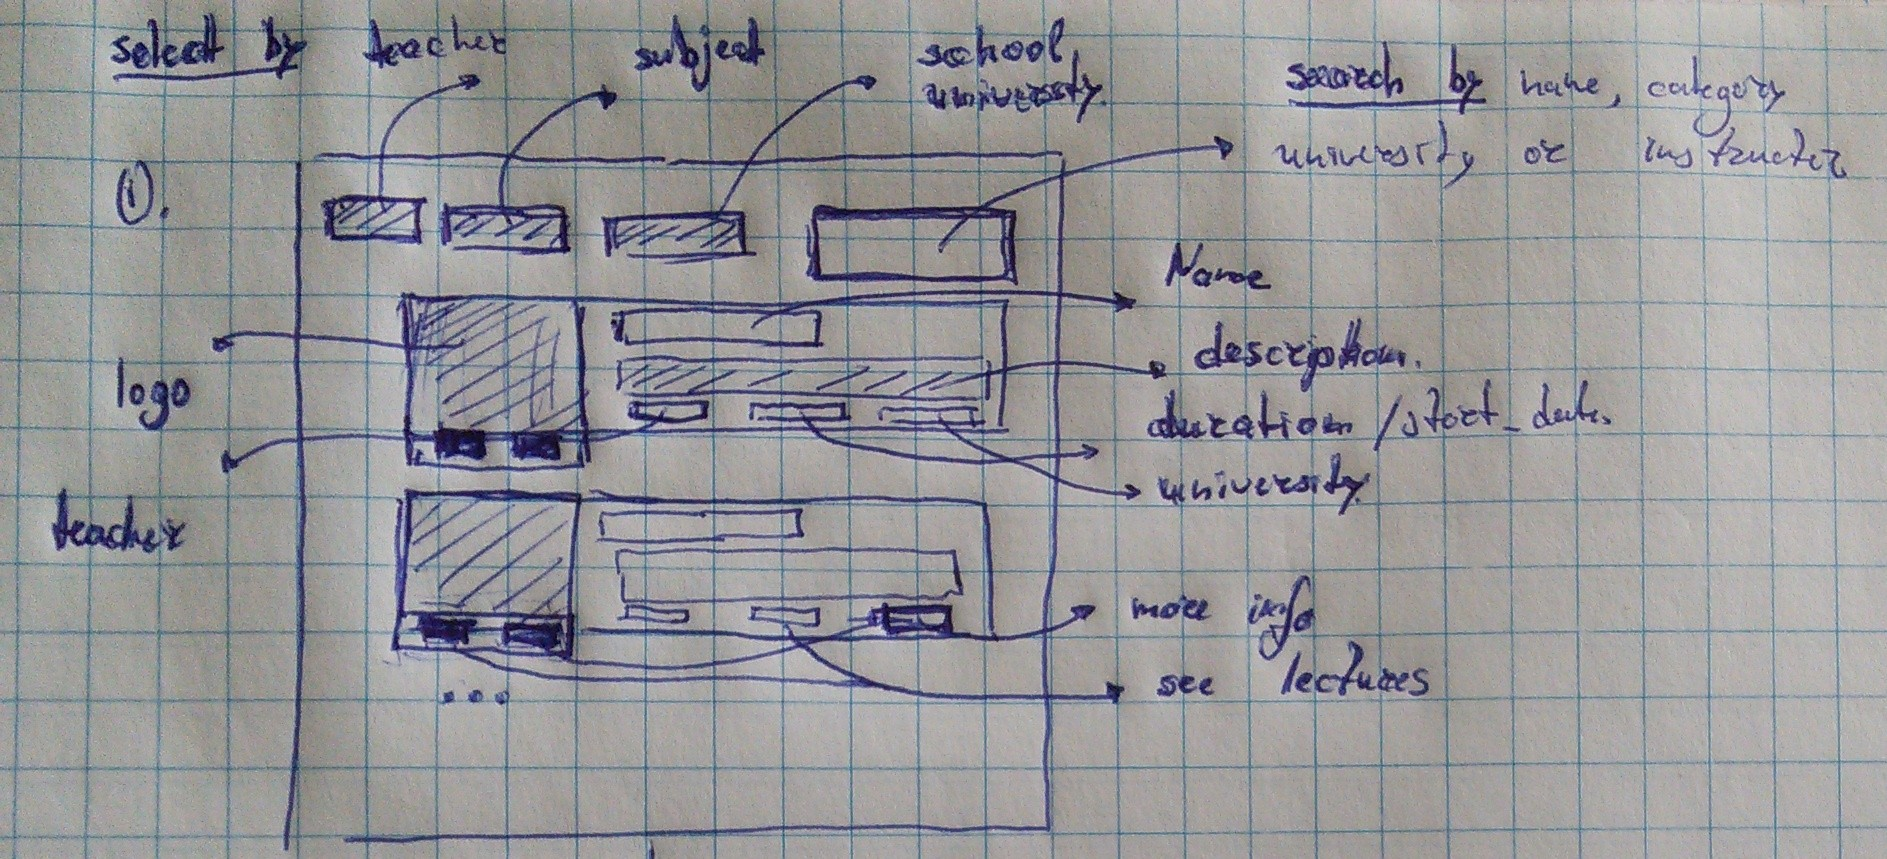
\includegraphics[width=0.8\textwidth]{img2}
   %       \\ Fig. 1. Index page
   %    \end{center}
   %  \end{minipage}

   The first page will contain a list of available courses, as you can see the
   top of the page will contain couple of \textit{select} boxes which allows to filter courses
  by teacher, subject/category. And a \textit{search} input by name, category, university or instructor. Thus by using
   this elements we responded to the first 2 questions in our list and allow users to search
   more faster for necesary course. \\

   Below there is a list of available courses. Each contains the \textit{name} of the course,
   a small \textit{description}, \textit{duration} of course,  the name of \textit{teacher}
   and \textit{university}. \\

   In the left part of each course is represented a logo, below it there are two buttons, \textbf{more info}
   and \textbf{see lectures}. This buttons will link to different pages, one is \textbf{about} page,
   and the other \textbf{lectures} page, in this manner we give the possibility to user to choose what he needs.

   \subsection{About page}

   This page contains information about the course, thus answering the 3-5th questions.
   Top of the page contains the name and the logo of it, in the right part it contains
   a small \textit{video} introduction if it exists, below is the description of the course
   followed by the name and photo of the teacher. And at the end of the page is included
   the necesary additional material that can be represented by a list of books or  a download link. \\

   In the right part there is a small list that contains: \textit{university name}, prerequisits,
   \textit{estimated time}, the \textbf{view lectures} button, and a small part of the comments,
   \textit{feedback} about course and a  link to \textbf{forum}.

   \subsection{Lectures page}

   This page contains the list of all lectures for a specific course. In the left part is a list
   of thumbnails of video with the name of the lecture. By clicking one of them in the right
   part will apear the video.

   Below it will be presented two buttons, \textbf{download} and \textbf{playback speed} button.
   Below the video there is of available topics discussed in the lecture, by clicking one of them the
   video will be forwarded to the time the topic is discussed.

   \vspace{0.5cm}

    \begin{minipage}[b]{1.0\linewidth}
      \begin{center}
        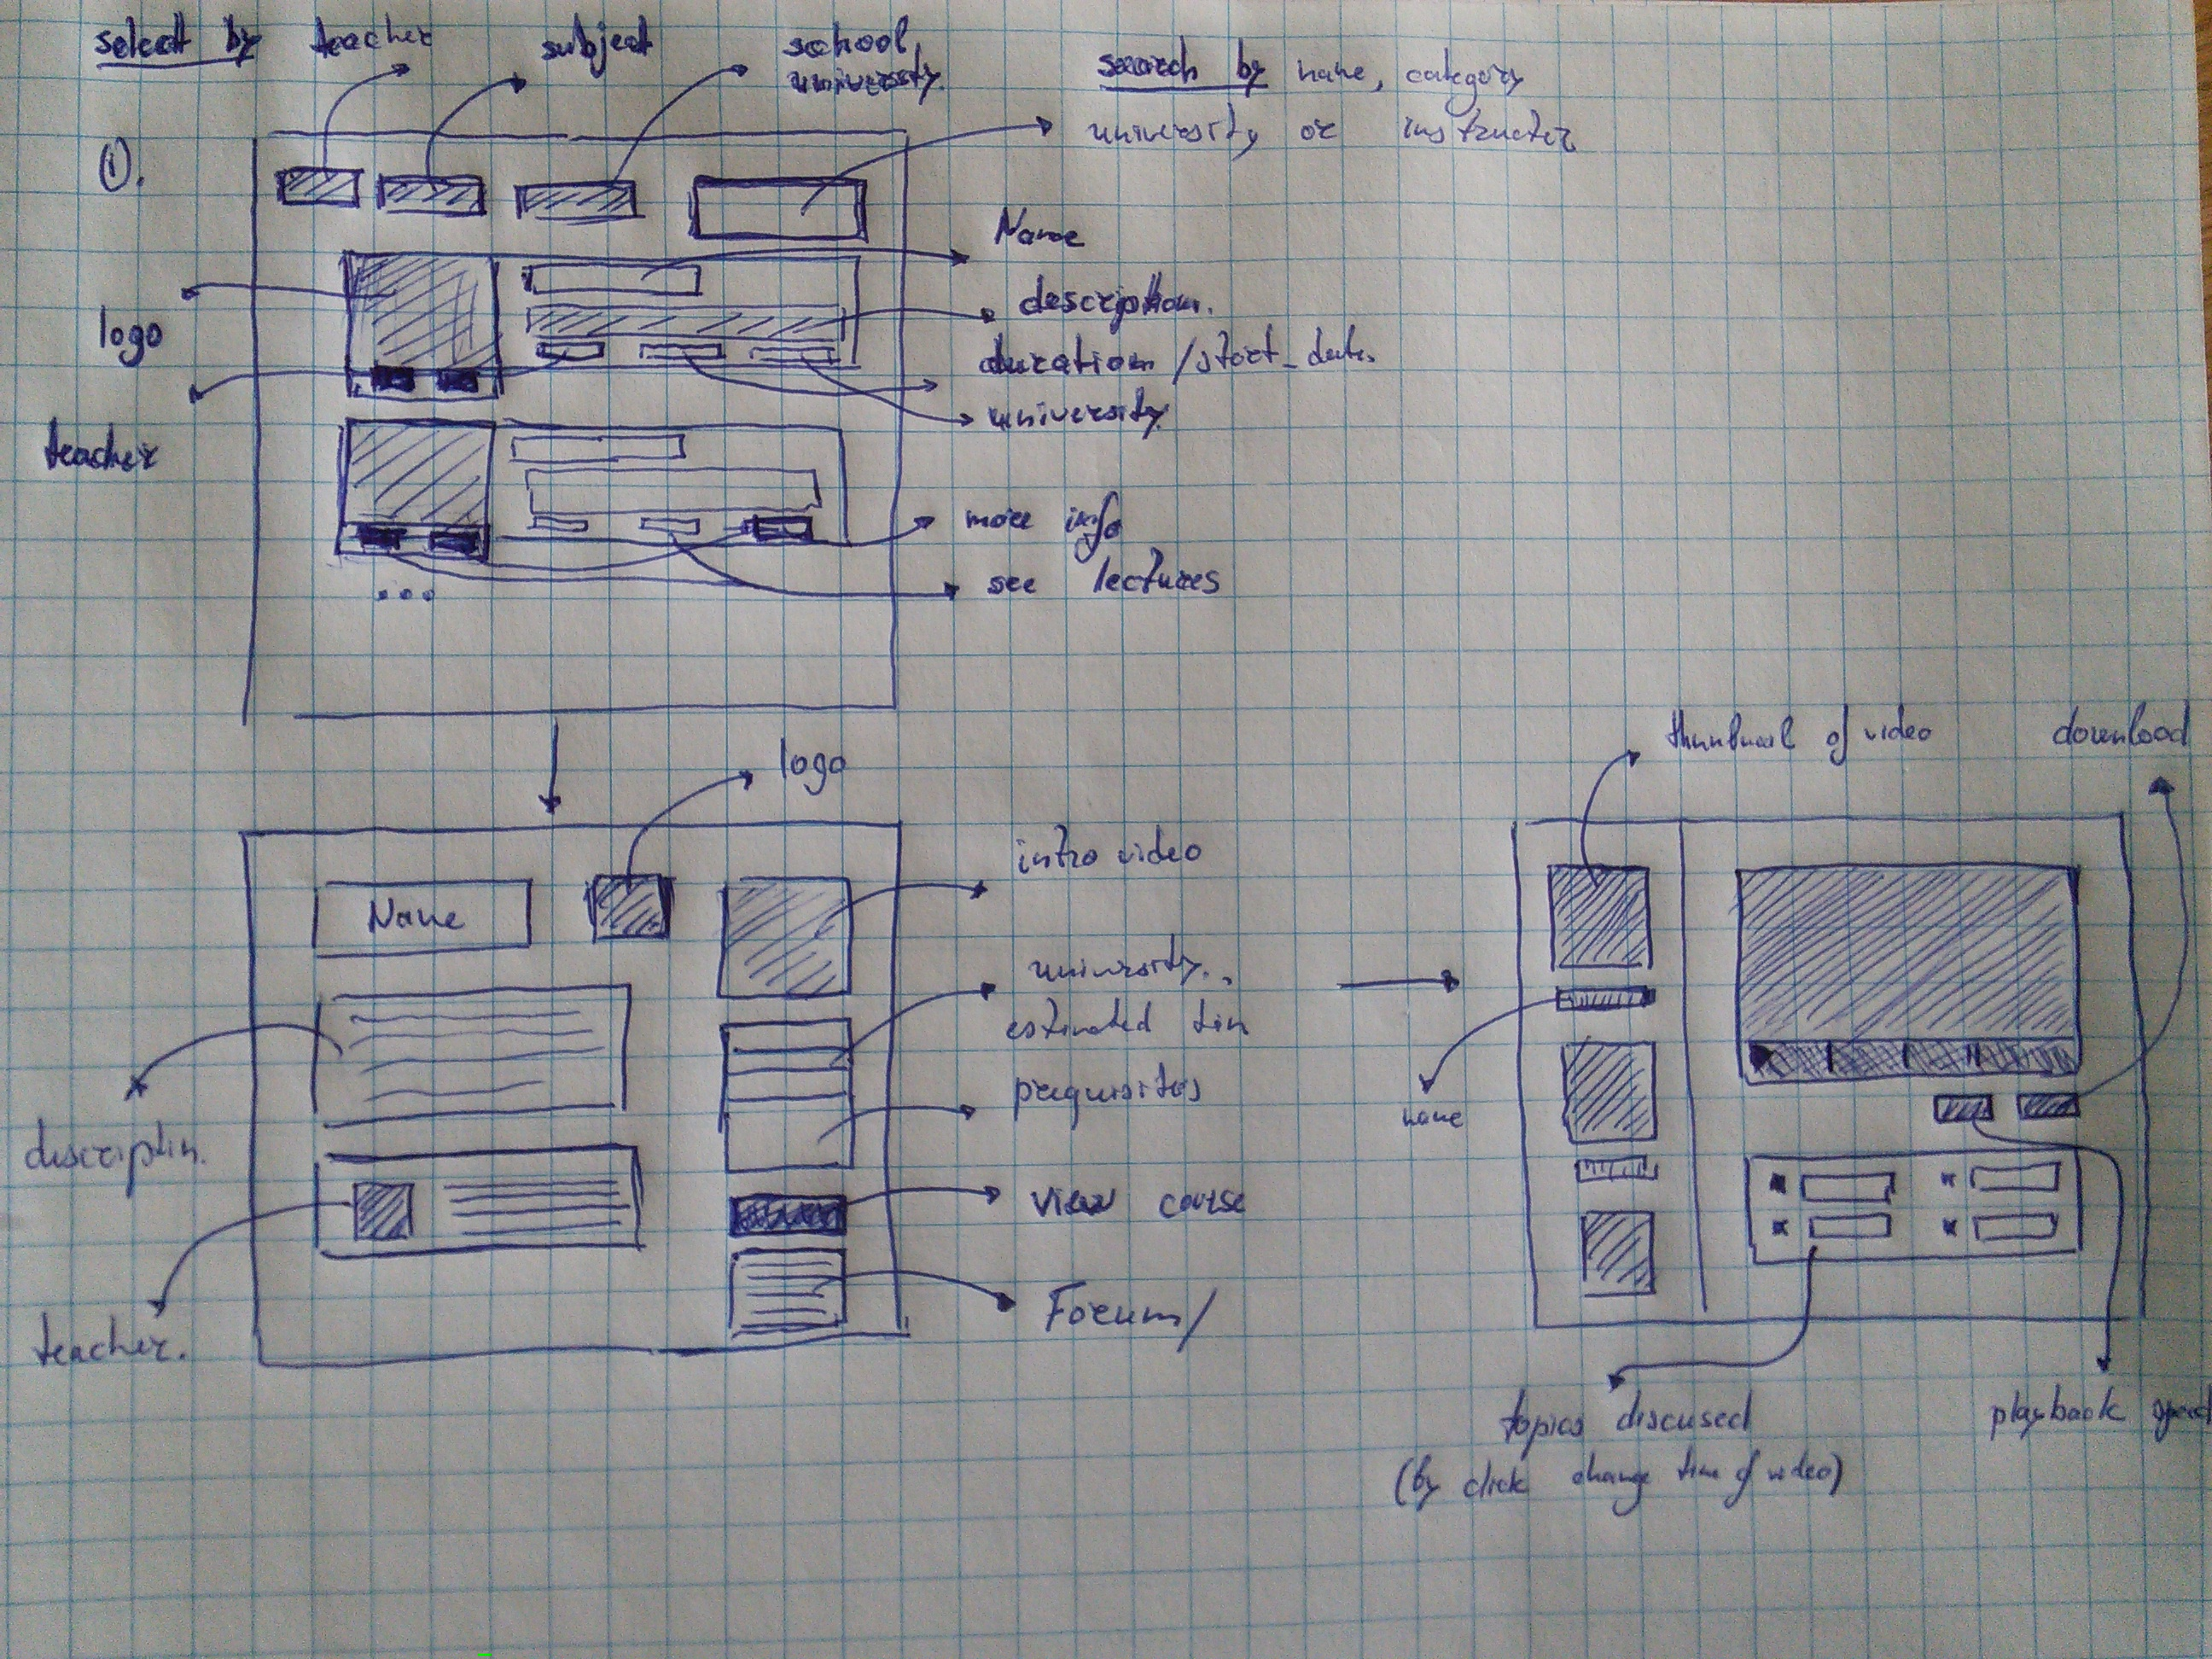
\includegraphics[width=0.9\textwidth]{img}
         \\ Fig. 1
      \end{center}
    \end{minipage}


\end{document}

